\documentclass[11pt]{article}

\usepackage[margin=1.0in]{geometry}
\linespread{1.5}
\usepackage{graphicx}
\usepackage{amsmath}
\usepackage{cite}

% definition of \customlabel, which is used to label supplementary figures and tables
\makeatletter
\newcommand{\customlabel}[2]{%
\protected@write \@auxout {}{\string \newlabel {#1}{{#2}{\thepage}{}{}{}}}}
\makeatother



\renewcommand{\bottomfraction}{.9}
\renewcommand{\topfraction}{.9}
\renewcommand{\textfraction}{0.1}
\renewcommand{\floatpagefraction}{.9}


\begin{document}

\section*{Introduction}

Over the years, a variety of models have been proposed to describe the effects of natural selection on protein-coding sequences. Traditionally, the focus has been on estimating the evolutionary rate ratio, $\omega = dN/dS$, the rate of nonsynonymous to synonymous substitutions, which indicates how quickly a protein's constituent amino acids change. Following early counting methods for estimating $dN/dS$ (e.g. refs \cite{LWL85} and \cite{NG86}), mechanistic codon substitution models (see ref.~\cite{Anisimova2009} for a comprehensive review) have taken a leading role as the inference method of choice since their introduction in the 1990s \cite{GoldmanYang1994, MuseGaut1994}. These so-called $\omega$ models have seen great success in the field of molecular evolution and are widely used to examine the strength of selection pressure in protein-coding sequences. 

More recently, a second class of models, known as mutation-selection-balance (MutSel) models, has emerged as a popular alternative to $\omega$ models. MutSel models explicitly model the dynamic balance between mutation and selection, lending a potentially more precise and realistic description of the evolutionary process than do $\omega$ models, which merely model the final outcome (e.g. substitution) of the underlying mutation-selection interplay \cite{HalpernBruno1998, YangNielsen2008, Rodrigueetal2010, Tamurietal2012}. Unlike $\omega$ models, MutSel models yield estimates of amino acid selection coefficients, which indicate the extent to which natural selection favors, or disfavors, particular amino acids at protein positions. These selection coefficients, which can in turn be scaled relative to a focal amino acid, the primary parameters of interest that MutSel models produce. Although MutSel models were first introduced over 15 years ago \cite{HalpernBruno1998}, they have seen virtually no use due to their high computational expense. However, recently, several computationally tractable model implementations have emerged \cite{RodrigueLartillot2014,Tamurietal2014}, allowing for the first time the potential for widespread use. 

Although both $\omega$ and MutSel models describe the same fundamental process of protein-coding sequence evolution along a phylogeny, it is largely unknown how these two classes of models relate to one another. In particular, as these inference methods have been developed independently, it remains an open question whether or not parameter estimates from one model are comparable to those of the other model. Therefore, while certain rhetorical arguments may be made in favor of using one method over another, there is currently no formalized, concrete rationale to guide researchers in their methodological choices. 

Here, we aim to formalize the relationship between $\omega$ and MutSel models by examining the extent to which their focal parameters, $\omega$ and scaled amino acid selection coefficients, yield overlapping information about the evolutionary process. To this end, we derive a mathematical relationship these models' primary parameters from which one can infer $\omega$ values from selection coefficients alone. Using a simulation approach, we verify that $\omega$ values estimated using selection coefficients alone correspond precisely to those inferred using the standard maximum likelihood $\omega$ inference approach. Further, we prove that, under conditions of symmetric mutation rates, this relationship holds only under regimes of purifying selection or neutral evolution ($dN/dS \leq 1$). This proof reveals that MutSel models are inherently unable to describe accurately protein evolution under a regime of positive diversifying selection, or when $dN/dS > 1$. This result has important implications for circumstances under which MutSel model use is justified.

Moreover, using this relationship as a benchmark, we have uncovered some potential biases inherent in $\omega$ inference methods. Typically, inference framework performance is assessed through simulating datasets which adhere to the underlying model's assumptions. However, this strategy can only confirm that inference methods are behaving as expected; it cannot confirm that the underlying model accurately represents the evolutionary process. Instead, we suggest an alternate approach to benchmark inference methods, and indeed evolutionary models: assessing the extent to which distinct models agree may serve as a novel, robust strategy to determine the accuracy of different modeling frameworks. 


\section*{Methods}

\subsection*{Sequence simulation and omega inference}
We simulated protein-coding sequences as a continuous-time Markov
process \cite{Yang2006} according to the MutSel model proposed by \cite{HalpernBruno1998}. This model's instantaneous rate matrix $Q = q_{ij}$, which describes the probability of substitution from codon $i$ to codon $j$, is given by 

\begin{equation}
Q_{ij} = \left\{ \begin{array}{rl}
              0                                           &\mbox{multiple nucleotide changes} \\
              f_{ij}\mu_{ij}                          &\mbox{single nucleotide transversion} \\
              f_{ij}\mu_{ij}\kappa               &\mbox{single nucleotide transition} \\
         \end{array} \right.,
\end{equation} where $\mu_{ij}$ is the symmetric nucleotide mutation rate and $f_{ij}$ is the fixation probability from codon $i$ to $j$. The fixation probability is defined as \begin{equation}f_{ij} = ln\bigg{(}\frac{\pi_j\mu_{ij}}{\pi_i\mu_{ji}}\bigg{)}\bigg{/}\bigg{(}1 - \frac{\pi_i\mu_{ji}}{\pi_j\mu_{ij}}\bigg{)},\end{equation} where $\pi_i$ is the equilibrium frequency of codon $i$.

For each simulation, we generated 20 scaled selection coefficients, $S_a$, by fixing one coefficient to 0 and drawing the remaining 19 values from a normal distribution $\mathcal(N)\sim(0,\sigma)$, where $\sigma ~ U(0.5, 1.5)$. We assigned these coefficients to codons such that all synonymous codons had the same scaled selection coefficient. Following the theory developed by \cite{SellaHirsh2005}, we determined steady-state codon frequencies $\pi_i$ according to \begin{equation} \pi_a = \frac{e^{S_i}}{\sum_k e^{S_k}}, \end{equation} where $S_i$ is the scaled selection coefficient for codon $i$ and the denominator sums over all 61 sense codons. 
 
We simulated protein-coding sequences along a 10-taxon phylogeny, with all branch lengths equal to 0.01, beginning with a root sequence selected using steady-state codon frequencies. Unless otherwise stated, we simulated alignments of 500,000 codon positions with a global, symmetric mutation rate $\mu_{xy} = 10^{-6}$, and a value for for $\kappa$ was drawn from $\mathcal{U} \sim (1,5.5)$. A single evolutionary model was applied to all positions in the simulated sequences, meaning that we did not incorporate any site-wise variation into the evolutionary process. While this lack of site-wise heterogeneity is unrealistic for real sequence evolution, it allows us to verify our derived relationship between selection coefficients and $\omega$ with a sufficiently sized data set.

Note that we additionally verified that the system was evolving under a state-state process by comparing the true codon frequencies with empirical codon frequencies calculated from the simulated alignment. The two sets of frequencies were virtually identical.

For each simulated alignment, we inferred $\omega$ in two main ways; first, we calculated $\omega$ using the mathematical framework described in \eqref{eq:fa}--\eqref{eq:dN}, and second, we inferred $\omega$ used the standard maximum likelihood M0 model \cite{NielsenYang1998}, which uses the GY94 rate matrix \cite{GoldmanYang1994}, as implemented in HyPhy \cite{KosakovskyPondetal2005}. The GY94 matrix includes the primary parameters $\omega$, $\kappa$, and equilibrium codon frequencies. As it is well-known that the manner of specification for the latter two parameters strongly influences $\omega$ estimates \cite{YN00, Yang2006}, we inferred $\omega$ under a variety of model parameterizations, including three $\kappa$ parameterizations ($\kappa$ fixed to 1, $\kappa$ fixed to its true value, and $\kappa$ as a free parameter), and four codon frequency specifications (equal codon frequencies,  F3x4 codon frequencies \cite{MuseGaut1994}, CF3x4 codon frequencies \cite{Pond2010} and empirical, or F61, codon frequencies \cite{GoldmanYang1994}). These different specifications yielded twelve maximum likelihood $\omega$ inferences per simulated alignment. All code used is freely available at \textbf{github}.


\section*{Results}


\section*{Mathematical relationship between selection coefficients and omega}


We describe here how to calculate $dN/dS$ from the parameters of a MutSel model. We assume the following: (i) the mutational process is symmetric, such that $\mu_{xy}=\mu_{yx}$ for all nucleotide pairs $xy$; (ii) all synonymous codons for a given amino acid have the same fitness (and therefore the same scaled selection coefficient); there is no synonymous rate variation or codon bias.

In the framework of a MutSel model, we can write the steady-state frequency of codon $i$ as
\begin{equation}\label{eq:pi_a}
 \pi_i=\frac{e^{S_i}}{\sum_k e^{S_k}},
\end{equation}
where the sum in the denominator runs over all 61 sense codons amino acids \cite{SellaHirsh2005}. Here, $S_i$ is the scaled selection coefficient for codon $i$; larger $S_i$ values correspond to higher frequencies of codon $i$. 

The fixation probability for a mutation from codon $i$ to codon $j$ is \cite{HalpernBruno1998,SellaHirsh2005}
\begin{equation}\label{eq:u_ij}
  u_{ij} = \frac{1-(\pi_i/\pi_j)^{1/N_e}}{1-\pi_i/\pi_j}
  \approx \frac{1}{N_e} \frac{\ln \pi_j - \ln \pi_i}{1-\pi_i/\pi_j}\,,
\end{equation}
where $N_e$ is the effective population size. We can calculate an evolutionary rate 
Using this framework, we can calculate an evolutionary rate by summing over all fixation probabilities weighted by the frequency of the originating codon. Further, we can establish expressions specifically for nonsynonymous and synonymous evolutionary rate, and then divide them in order to obtain a value for the evolutionary rate ratio $dN/dS$.

For example, we can write the synonymous rate $K_\text{S}$ as
\begin{equation}\label{eq:KS}
  K_\text{S} = N_e \sum_i \sum_{j \in {\cal S}_i} \pi_i  u_{ij}\mu_{ij}\,,
\end{equation}
where ${\cal S}_i$ is the set of codons that are synonymous to codon $i$ and differ from it by one nucleotide substitution. To normalize $K_\text{S}$, we divide it by the number of synonymous sites, which we calculate according to the mutational opportunity definition of a site \cite{GoldmanYang1994, Yang2006} as 
\begin{equation}\label{eq:LS}
  L_\text{S} = \sum_i \sum_{j \in {\cal S}_i} \pi_i \mu_{ij},.
\end{equation}
Under the assumption that all synonymous codons have equal fitness, and hence all synonymous mutations are selectively neutral, we have $u_{ij}=1/N_e$ \cite{CrowKimura1970}, and thus we find that $dS$, the synonymous rate per synonymous site, is equal to 1.

Similarly, we can derive an expression for $dN$, the non-synonymous rate per non-synonymous site, and we find
\begin{equation}\label{eq:dN}
  dN = \frac{K_\text{N}}{L_\text{N}}=\frac{ N_e \sum_i \sum_{j \in {\cal N}_i} \pi_i u_{ij} \mu_{ij} } {\sum_i \sum_{j \in {\cal N}_i} \pi_i \mu_{ij} },
\end{equation}
where ${\cal N}_i$ is the set of codons that are nonsynonymous to codon $i$ and differ from it by one nucleotide substitution. The quantities $K_\text{N}$ and $L_\text{N}$ are defined as in Eqs.~\eqref{eq:KS} and \eqref{eq:LS} but summing over $j\in {\cal N}_i$ instead of $j\in {\cal S}_i$. Equations \eqref{eq:pi_i}--\eqref{eq:dN} establish a connection between the scaled amino acid selection coefficients $s_a$ (i.e., the primary parameters of a MutSel model) and the evolutionary rate ratio $dN/dS$. 


\subsection*{Scaled selection coefficients fully encapsulate $\omega$}

To validate our derived relationship between scaled selection coefficients and $\omega$, we simulated protein-coding sequences along a 10-taxon phylogeny according to the Halpern-Bruno mutation-selection model \cite{HalpernBruno1998}, assuming no codon bias and symmetric nucleotide mutation rates. We calculated an $\omega$ for each simulated alignment using the derivations given in equations \eqref{eq:pi_i}--\eqref{eq:dN} as well as standard (ML) methods, according to the GY94 \cite{GoldmanYang1994} rate matrix, as implemented in the HyPhy batch language \cite{KosakovskyPondetal2005}.

As shown in Figure~\ref{reg_conv}A, $\omega$ values derived using selection coefficients agree nearly perfectly with those inferred using standard maximum likelihood methods. We additionally demonstrate convergence of these values with increasing amounts of data, represented by simulated alignment length (Figure~\ref{reg_conv}B). Taken together, these results clearly show that MutSel model parameters fully encapsulate information regarding the evolutionary rate ratio, $\omega$, and that the results from MutSel and $\omega$ models are largely in agreement. 

Moreover, as seen in Figure~\ref{reg_conv}A, estimates for $\omega$ never exceed 1, but rather all reflect a regime of purifying selection. In fact, in SuppMat, we prove that, when calculated using scaled selection coefficients, $\omega$ is necessarily always less than or equal to 1. This important insight reveals that, while MutSel models fully agree with $\omega$ models, this relationship only holds under conditions of purifying selection or neutral evolution. MutSel models, therefore, are inherently unable to describe protein evolution under positive, diversifying selection ($\omega > 1$).



\subsection*{Influence of ML model parameterizations}

ML $\omega$ values reported in the previous subsection were obtained by fixing $\kappa$ parameter in the GY94 rate matrix to its true simulated value, and specifying equal codon frequencies. However, it is well-known that different ML parameterizations can influence its $\omega$ estimation \cite{YN00,Yang2006,ZhangYu2006}.  Therefore, we additionally inferred ML $\omega$ values according to 11 other model parameterizations. Specifically, we inferred $\omega$ when $\kappa$ was either a free parameter of the model, fixed to its true value, or fixed to 1, and we examined different equilibrium codon frequency specifications, including equal codon frequencies, frequencies calculated using either the F3x4 \cite{MuseGaut1994} or the CF3x4 \cite{Pond2010} estimators, or empirical codon frequencies as taken from the simulated alignment. Table~\ref{tab:mlspec} shows how the $\omega$ values estimated according to these different ML parameterizations relate to the $\omega$ values as calculated using equations \eqref{eq:pi_i}--\eqref{eq:dN}. 

Several important insights into the behavior of ML $\omega$ models can be gained from these results. First, it is clear that equal codon frequencies dramatically outperform all other specifications. Under this frequency specification, ML also estimates $\kappa$ fairly accurately while maintaining an extremely high $\omega$ correlation of 0.993. Second, the F3x4 and CF3x4 frequency estimators perform nearly identically to one another, and neither frequency specification estimates $\omega$ values which correlate with our derived $\omega$. Finally, when empirical codon frequencies are used, $\omega$ estimates have a moderately strong, negative correlation. In fact, under this frequency specification, ML $\omega$ values are dramatically inflated, as illustrated in Figure~\ref{reg_fspec} (plots showing all regressions are in Figure~\ref{fig:reg_allspecs}). As we have proven that, when calculated from scaled selection coefficients, $\omega$ is necessarily less than or equal to 1, we interpret the use of F3x4 or empirical codon frequencies effectively as ML model misspecifications, leading to grossly elevated $dN/dS$ values. However, it is interesting to note that, while ML yields the most accurate $\kappa$ estimates when codon frequencies are set to $1/61$ each, all frequency specifications yield $\kappa$ estimates which correlate relatively strongly with the true $\kappa$ values. Thus, the ML model's ability to accurately estimate $\kappa$ appears much more robust to codon frequency specifications is than its ability to estimate $\omega$.

%Additionally, the error between our derived $\omega$ and the ML $\omega$ estimate scales well with the extent of selection pressure. Something about how entropy correlates well with omega, too, like r=0.91. this makes sense. more constraint because fewer codons are allowed. however the opposite sort of happens with ml inference - more constraint, more elevated values. While way less of an issue than with f3x4 or empirical freqs, also occurs with equal freqs. The question is, is this a problem for real analyses? Probably not terribly, but it might be.

Thus, the question emerges of why specifying equal codon frequencies leads to precisely accurate $dN/dS$ estimates, whereas the other, more commonly used specifications produce incorrect and biased estimates. The basis for including codon frequencies in mechanistic codon substitution models is to capture biases in the underlying nucleotide base frequencies \cite{YN00, Yang2006}. Indeed, our simulations produced alignments with a wide array of GC-content values (ranging from ??? - ??? ), yet the GC-content had no effect on $\omega$ correlations (p = ???,when lm(derived~ml+gc)). Importantly, as we adopted symmetric mutation rates in our simulations, these varying degrees of GC-content were not caused by any bias towards unequal base frequencies, but rather by codon fitness differences alone. Thus, the correct frequencies to specify in ML inference should reflect those frequencies which would be present \textit{in the absence} of selection, which, the case of symmetric mutation rates, corresponds to equal codon frequencies.

So, it is critical to parameterize models properly in order to be confident that $\omega$ is the sole parameter representing selection. If, as is the case when non-equal freqs were specified, other parameters in the model take on an interpretation of selection, then $\omega$ is not going to mean what we naively assume it must.
Highlights potential issues with the $\omega$ class of models. While the framework for $dN/dS$ is one rooted in popgen, these markov processes are not. MutSel models, on the other hand, use a markov process explicitly based on the underlying population genetics principles governing the evolutionary process. 


In conclusion, when diffs in gc-content are driven by mutational processes alone, we are mostly ok. when, however, selective forces contribute to compositional, for instance by favoring gc-rich codons, inference is wacky, but best when equal frequencies are specified. Thus, we see no reason to continue including this parameter, at least in cases of purifying selection. Although we are able to test only ML performance when evolving under steady-state, we also suspect that eq freqs shouldnt be there for positive selection either, because if positive selection is happening then clearly the system is not at equilibrium and thus using steady-state codon frequencies is a logical flaw.




Important result from our study was the methodological approach of benchmarking ML methods. This is not typically how benchmarking is done, but probably represents something very robust. The specific approach here is somewhat limited; 



%In verifying the derived relationship between selection coefficients and $dN/dS$, we encountered some biases in ML inference methods. In particular, the specific codon frequency specification that the ML inference used had a substantial effect on its accuracy. Only when specifying equal codon frequencies (an equilibrium frequency of $1/61$ for each codon, regardless of that codon's actual frequency in the given data set) were we able to achieve agreement between our derived and ML $dN/dS$ estimates (Figure~\ref{freqspec_compare}) . On the other hand, when more commonly used codon frequency specifications, included the popular F3x4 estimator and simply using frequencies as measured from the data, ML yielded strongly inflated $dN/dS$ estimates. Indeed, as the model's codon frequency parameters were more and more tailored to the given data set, error between derived and ML $dN/dS$ values increased.

%Importantly, however, our simulated data sets contained relatively constrained amino acid, and thus codon, frequencies, as a single MutSel  parameterization was applied to all positions in the simulated alignment. Therefore, we examined the extent to which codon constraints influenced this tendency for frequency specifications to yield spurious results. For each simulated alignment $i$, we calculated the Shannon entropy, \begin{equation} H(i) = - \sum_j P_j \ln P_j \end{equation}, where $P_j$ is the frequency of codon $j$ and the sum runs over all sense codons. Note that, for sense codons, the maximum $H(i) = 4.11$ value is reached when all codons have a frequency of $1/61$. We then examined the relationship between error in $dN/dS$ estimates caused by different codon frequency specifications and alignment codon entropy, as shown in Figure~\ref{reg_fspec}. Clearly, as entropy increases, thus approaching a flatter distribution of codon frequencies, error in ML estimates does indeed decrease. Even so, specifying equal codon frequencies will nearly always minimize the error.

We have two possible explanations for this trend.
The first is that these results reflect a broad misinterpretation of how the equilibrium codon frequencies parameters should be specified in mechanistic codon models. Typically, these values are taken directly from the given data and fixed in the model to reduce the number of parameters inferred. However, the codon frequencies observed in the data set represent those which exist \textit{after} natural selection has acted on the sequence. Instead, the model should use the codon frequencies which would exist \textit{in the absence of natural selection}. Selection, alternatively, acts to tune this frequencies to increase protein fitness. If one specifies equilibrium frequencies which exist after natural selection has acted on the protein sequence (i.e., frequencies measured directly from the data), then the influence of selection pressure is incorporated into these values. The desirable outcome, however, is that the $dN/dS$ parameter measures the selective strength. If other parameters in this model contain selection information, estimates for $dN/dS$ will not accurately capture selective effects.

The second explanation is that a single parameter $dN/dS$ is in effect representing two distinct values; on one hand, $dN/dS$ indicates the strength of selective constraint. On the other hand,  

% Inference from molecular sequence data is a mature field, and wide variety of different inference frameworks have been developed to study selection on protein-coding genes. The oldest and most-widely used one calculates the ratio of non-synonymous ($dN$) to synonymous ($dS$) substitution rates $dN/dS$ to identify sites that experience negative selection ($dN/dS<1$), sites that evolve neutrally ($dN/dS\approx1$), and sites that experience positive diversifying selection ($dN/dS>1$). By contrast, MutSel models aim to estimate selection coefficients, either for individual amino acids \cite{HalpernBruno1998,Bruno1996,Rodrigueetal2010,Tamurietal2012,Tamurietal2014}, for codons \cite{YangNielsen2008}, or for both. Other approaches calculate overall substitution rates and attempt to distinguish rapidly from slowly evolving sites (rate models, e.g.~\cite{Pupkoetal2002,HuangGolding2014}), or describe the biophysical processes by which specific amino acids are replaced by other amino acids (exchangeability models, e.g.~\cite{Kosioletal2007,Conantetal2007,Conantetal2009,Delport2010}).

%Researchers interested in applying these methods to their study system of choice thus find that they have a bewildering array of different methods at their disposal. Which specific method to choose is often not obvious, and frequently researchers simply pick the methods they believe will work best on their data, without having any solid evidence to support this belief. The problem of model choice is compounded by a lack of understanding of how different modeling frameworks perform on the same data. If we analyzed a data set with Model B instead of Model A, would we have gotten a comparable answer? Do Models A and B give predictions that generally agree, or are there data sets where they produce conflicting inferences? 



\subsection*{Discussion}

% summary paragraph
Here, we have derived a formal mathematical relationship between the parameter estimates of MutSel and mechanistic codon models. Through a simulation approach, we validated this relationship and demonstrated that these models yield nearly identical results. However, we additionally found that MutSel models necessarily cannot describe scenarios in which positive or diversifying selection occurs, or when $dN/dS > 1$. Although it is generally acknowledged that MutSel models carry the assumption of purifying selection, we formalize and prove this result. These findings have important implications for how and when these models should be applied. In cases of purifying selection or neutral evolution, these two competing models are virtually no different from one another, and thus use of either model is fully justified. Alternatively, if positive selection is occurring, MutSel models cannot be used as they mathematically cannot capture the actual evolutionary process.

% why this study was good
This study highlights the importance of examining the similarities and differences among different evolutionary model classes. While some may prefer one model over another, it is important to have a full understanding of why one model might be applied over another. Our results demonstrate that, for circumstances of purifying selection or neutral, the models are robust and in agreement. However, be careful, because sometimes they don't agree, and this is equally important.

%implications for future model use.

% parameterization implications for future stuff
Now, for the frequency specification: does this really matter? Typically, when one measures codon frequencies from the data set, codon frequencies are treated as global parameters rather than site-specific. Thus, equilibrium codon frequency parameters effectively represent an average across the entire data set, naturally lead to a flatter distribution of codon frequencies. Our simulated data sets, on the other hand, were evolved according to a single parameter site, leading to more constrained global codon frequencies. Therefore, the extent to which bias introduced by incorrect frequency specifications was driven by how far from equal we're talking.

%any study problems
Caveat about how our math relies on symmetric mutation rates and/or equal mutation rates, depending on which one ends up happening.
	

%\subsection*{Mutation-selection-balance models are only valid for purifying selection}

%\textbf{I really have no idea how to write up proofs, so I've virtually just latex'd the mathematica document. But at least the equations are there! ... next day: I'd better stop. This section might have to be yours, unfortunately.}

%To show that mutation-selection models only corresponds to $dN/dS \leq 1$, we make use of that fact that each calculation of $dN/dS$, as described in equations \eqref{eq:pi_a}--\eqref{eq:dN}, entails summing the forward and backward fixation probabilities between codons, which are in turn divided by the codon frequency sums. We additionally assume that all mutation rates $\mu_{ij}$ are equal, and as all values for $N$ will ultimately cancel, we exclude them from the following proof. We will deal with the case of two nonsynonymous codons, $i$ and $j$, and we write their frequencies as $x$ and $y$, respectively.

%As follows from \eqref{eq:pi}, the sum of the probabilities going from codon $i$ to codon $j$ and from codon $j$ to codon $i$ is \begin{equation} xP(x,y) + y(P(y,x) = \frac{2xy [\ln x - \ln y]}{x - y}\end{equation}, and we will demonstrate that this value is necessarily $\leq x + y$ for $x,y \geq 0$ and $x \leq y$.

%To this end, we define the function \begin{equation} F(x,y) = x + y - \frac{2xy [\ln x - \ln y]}{x - y} \end{equation}. Thus, we show that $F(x,y) \geq 0$. For the condition $x=y$, this is straightforward to show, as $\lim_{x \to y}F(x,y) = 0$. 
%We now show that the first derivative of $F(x, y)$ is negative throughout $x \in (0,y)$, thus proving that $F(x, y)$ has to be monotonically decreasing, and hence $\geq0$, in this interval.

%dNdS limitations:
%One such limitation is that the $dN/dS$ parameter ignores the influence of site-specific amino acid propensities.  It is universally recognized that a particular position in a protein will only tolerate certain amino acids, due either to functional or structural constraints. However, $dN/dS$ ignores this key aspect of protein evolution and considers all nonsynonymous changes, regardless of which amino acid was substituted, as having equal weight on protein fitness, a biologically implausible assumption. An additional limitation is that codon-substitution models merely describe the result of the evolutionary process, rather than the explicit underlying mechanism producing those results. More precisely, substitutions in protein-coding sequences result from an ongoing mutation-selection balance. When a mutation occurs in a DNA sequence, natural selection must act on this mutation, either by disfavoring it, resulting in the mutation's removal from the population, or favoring it, ultimately yielding an amino acid replacement or substitution. By overlooking this underlying mechanism and focusing only on whether substitutions have occurred, codon substitution models are unable to capture the full extent of the evolutionary process. 

	
\newpage
\bibliographystyle{plos2009}
\bibliography{bibliography}	

\begin{figure*}[H]
\centerline{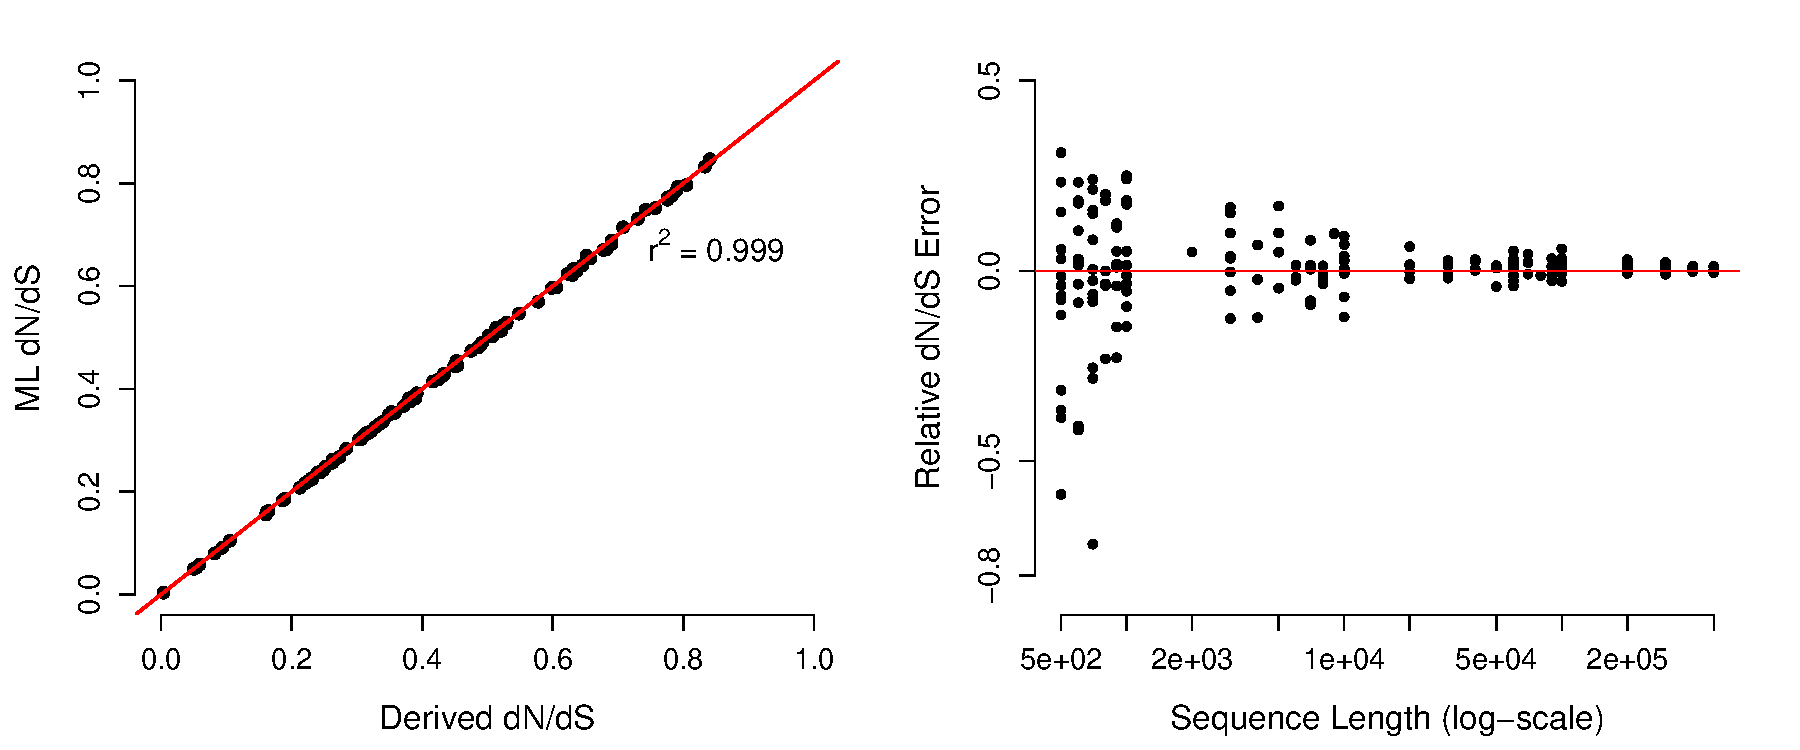
\includegraphics[width=5in]{figures/regression_convergence.pdf}}
\caption{\label{reg_conv} Relationship works exceedingly well. Left panel shows 100 points, each of which corresponds to single simulation. Note that here the ml inference is shown for equal codon frequency specs and kappa fixed to true value (a similar plot for free kappa is shown in suppfigs, but results are qualitatively identical.) Right panels shows convergence of omega values as data set size (represented as simulated alignment length) increases. The y-axis indicates relative error of the ML $dN/dS$ estimates, and the x-axis indicates sequence length on a log-scale. As the sequence length, or the data set size, increases, the two $dN/dS$ estimates converge to the same value. }
\end{figure*}

	

\begin{table}[htbp]
\caption {\label{tab:mlspec}Effect of ML parameterizations on inference.}
\begin{tabular}{c c c c c c}
\hline\noalign{\smallskip}
\multicolumn{1}{l}{Codon frequencies} & \multicolumn{1}{l}{$\kappa$ parameterization} & \multicolumn{1}{l}{$\omega$ correlation} &\multicolumn{1}{l}{$\omega$ error} & \multicolumn{1}{l}{$\kappa$ correlation} &\multicolumn{1}{l}{$\kappa$ error} \\
\hline\noalign{\smallskip}
Equal & True & 0.999 & 0.008 &   &   \\ % the 1.0 is 0.9997 
Equal & 1 & 0.916 & 0.195 &   &   \\ 
Equal & Free & 0.996 & 0.023 & 0.913 & 0.106 \\ 
\hline\noalign{\smallskip}
F3x4 & True & -0.276 & 1.696 &   &   \\ 
F3x4 & 1 & -0.233 & 1.317 &   &   \\ 
F3x4 & Free & -0.278 & 1.727 & 0.929 & 0.141 \\ 
\hline\noalign{\smallskip}
CF3x4 & True & -0.301 & 1.718 &   &   \\ 
CF3x4 & 1 & -0.259 & 1.317 &   &   \\ 
CF3x4 & Free & -0.301 & 1.747 & 0.932 & 0.136 \\ 
\hline\noalign{\smallskip}
Empirical & True & -0.648 & 10.09 &   &   \\ 
Empirical & 1 & -0.629 & 7.992 &   &   \\ 
Empirical & Free & -0.656 & 10.29 & 0.804 & 0.227 \\ 
\noalign{\smallskip}\hline\noalign{\smallskip}
\end{tabular}
\newline
Codon frequency specifications were either set as equal (1/61 per codon), calculated from the F3x4 estimator \cite{MuseGaut1994}, calculated from the CF3x4 estimator \cite{Pond2010}, or set equal to the simulated alignment's empirical frequencies. $\kappa$ was specified as either a fixed value, its true simulated value or 1, or as a free parameter of the model. Correlations given are between the ML $\omega$ estimate and our derived $\omega$ values. Error refers to the mean absolute error between these two $\omega$ estimates. Similar values for $\kappa$ are shown for those inferences where $\kappa$ was a free parameter of the model. Note that all is significant.
\end{table}	
	

\bigskip
\begin{figure*}[H]
\centerline{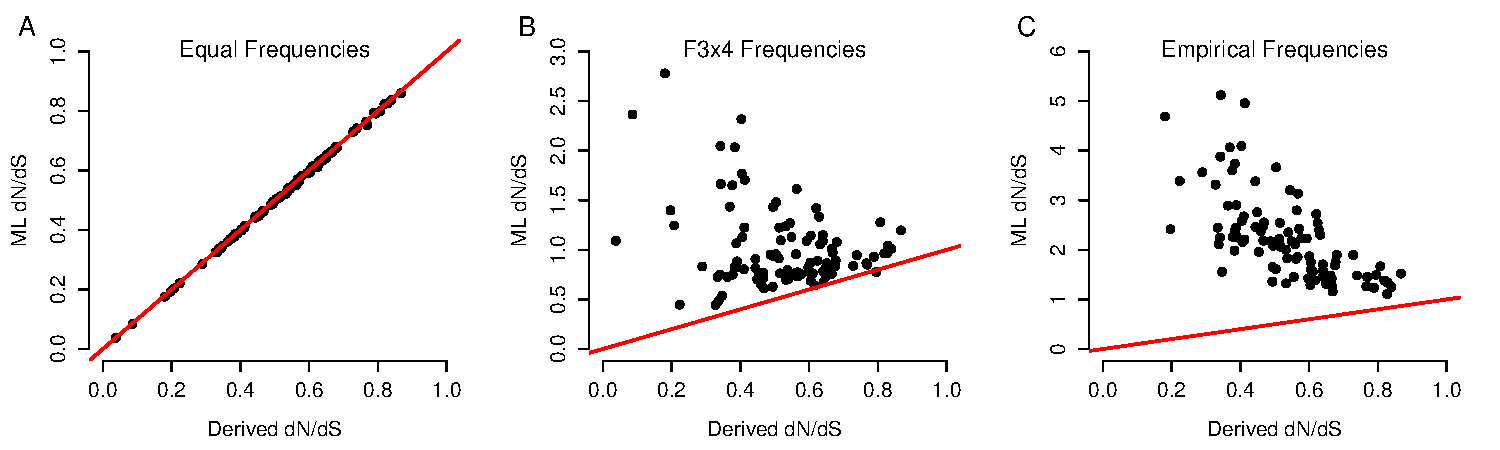
\includegraphics[width=6in]{figures/regression_fspec_kappatrue.pdf}}
\caption{\label{reg_fspec} Issues with frequency specifications abound. In each plot, red line indicates 1:1 agreement, so note the y-axis differences. Relationship between omega values only really exists when equal codon frequencies are specified. When f3x4 or true freqs used, there is the potential to end up with dramatically inflated values. cf3x4 not shown because its results are statistically the same as f3x4.}
\end{figure*}



\clearpage
\newpage

\section*{Supplementary Figures}

\centerline{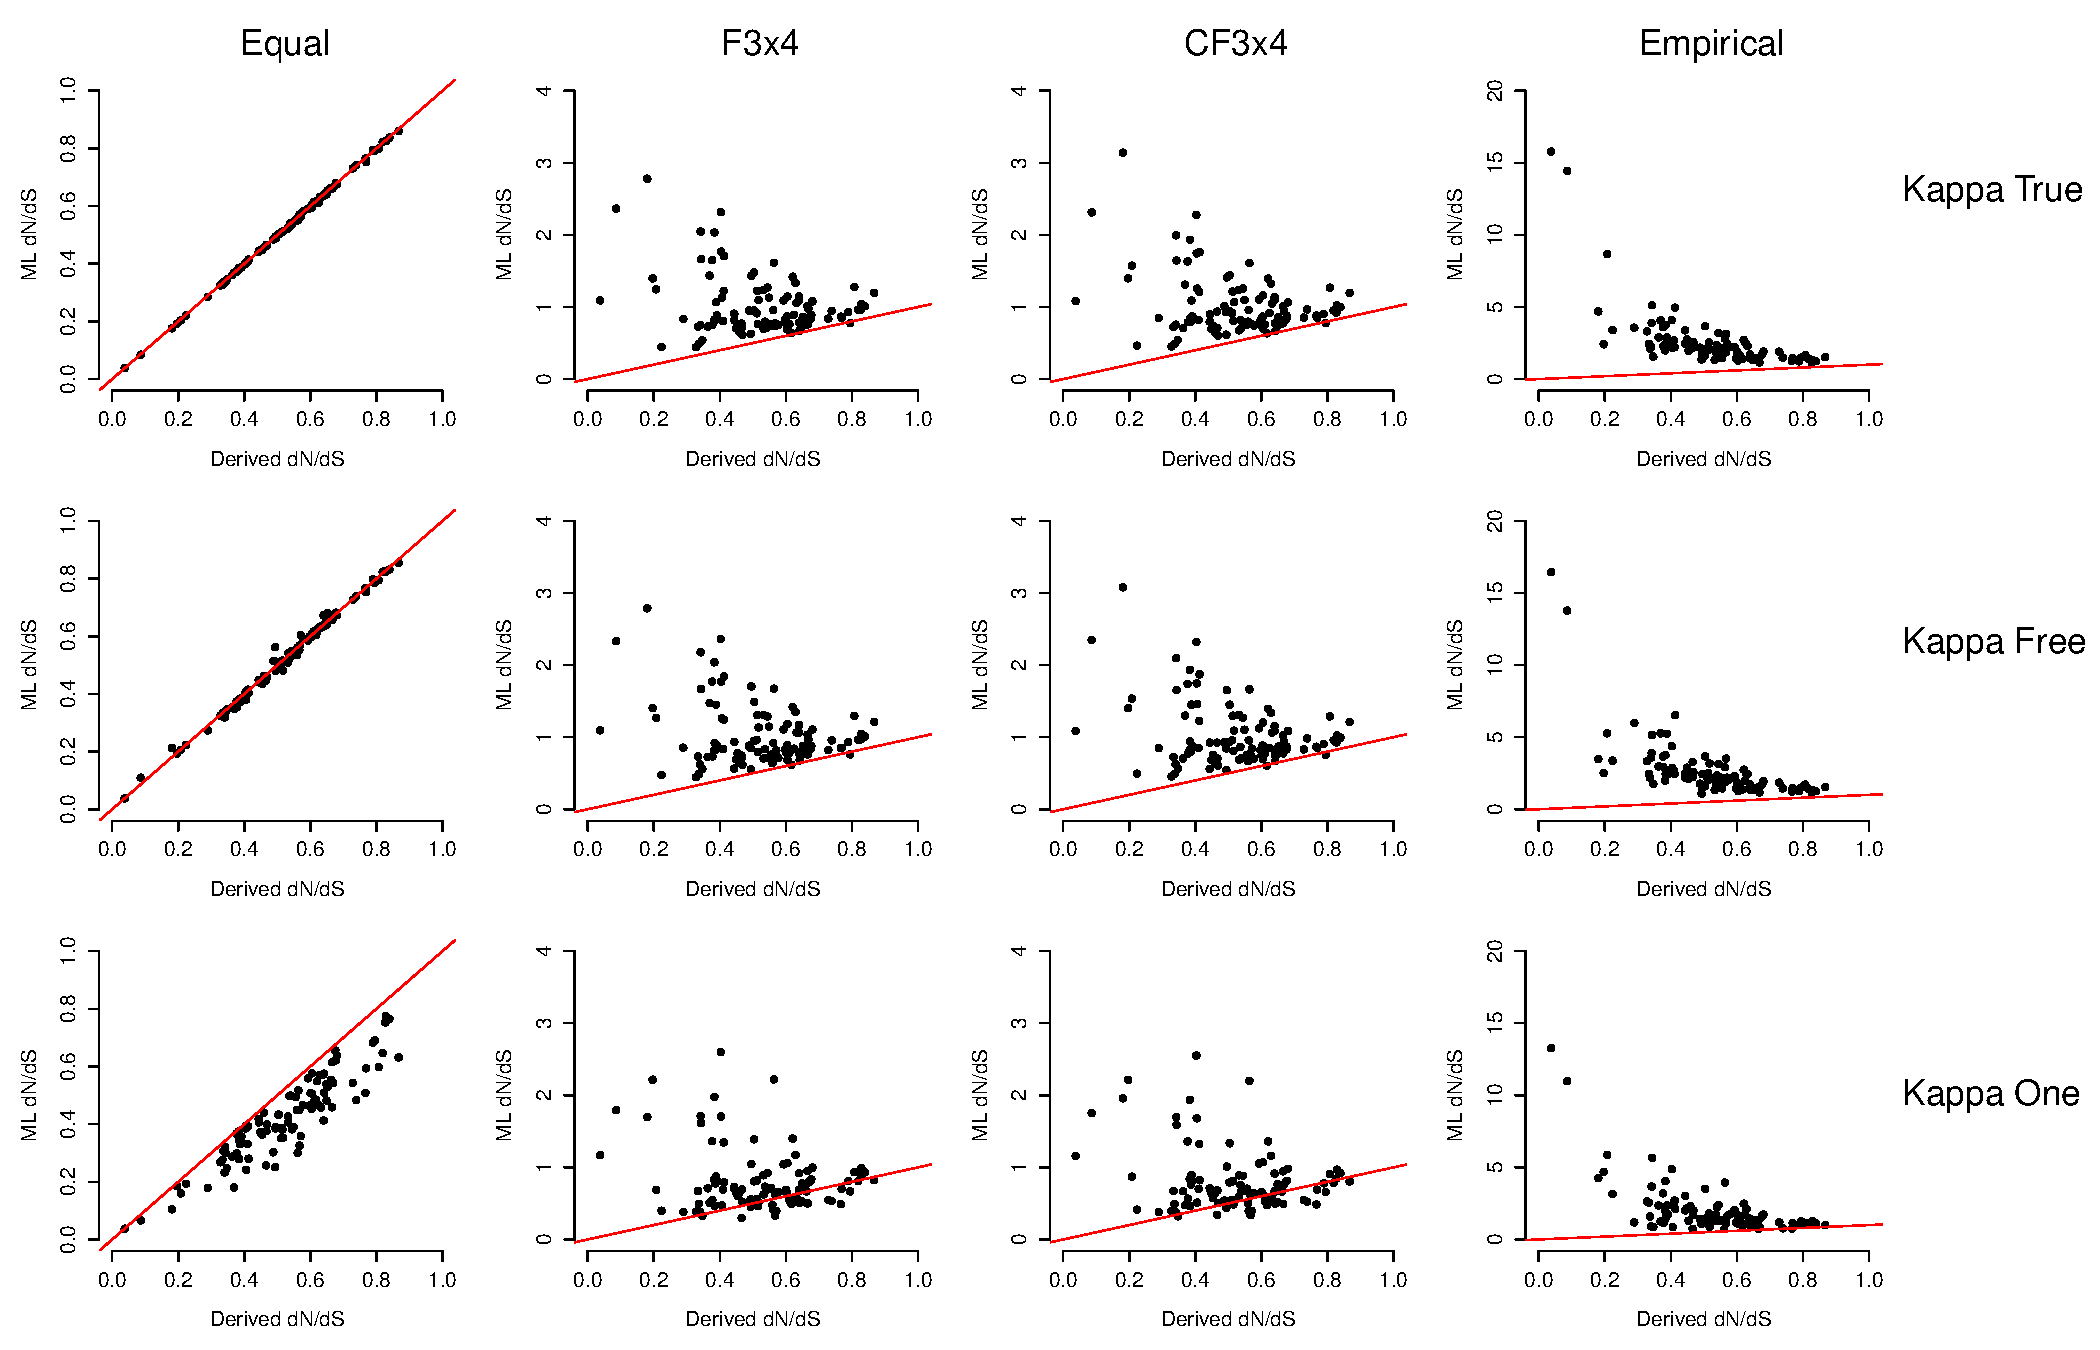
\includegraphics[width=6in]{figures/regression_allspecs.pdf}}
\noindent \textbf{Fig. S1} Regression for all ML parameterizations.
\customlabel{fig:reg_allspecs}{S1}

\end{document}

